\begin{figure}
    \centering
    % \begin{subfigure}[b]{0.49\textwidth}
    %     \centering
    %     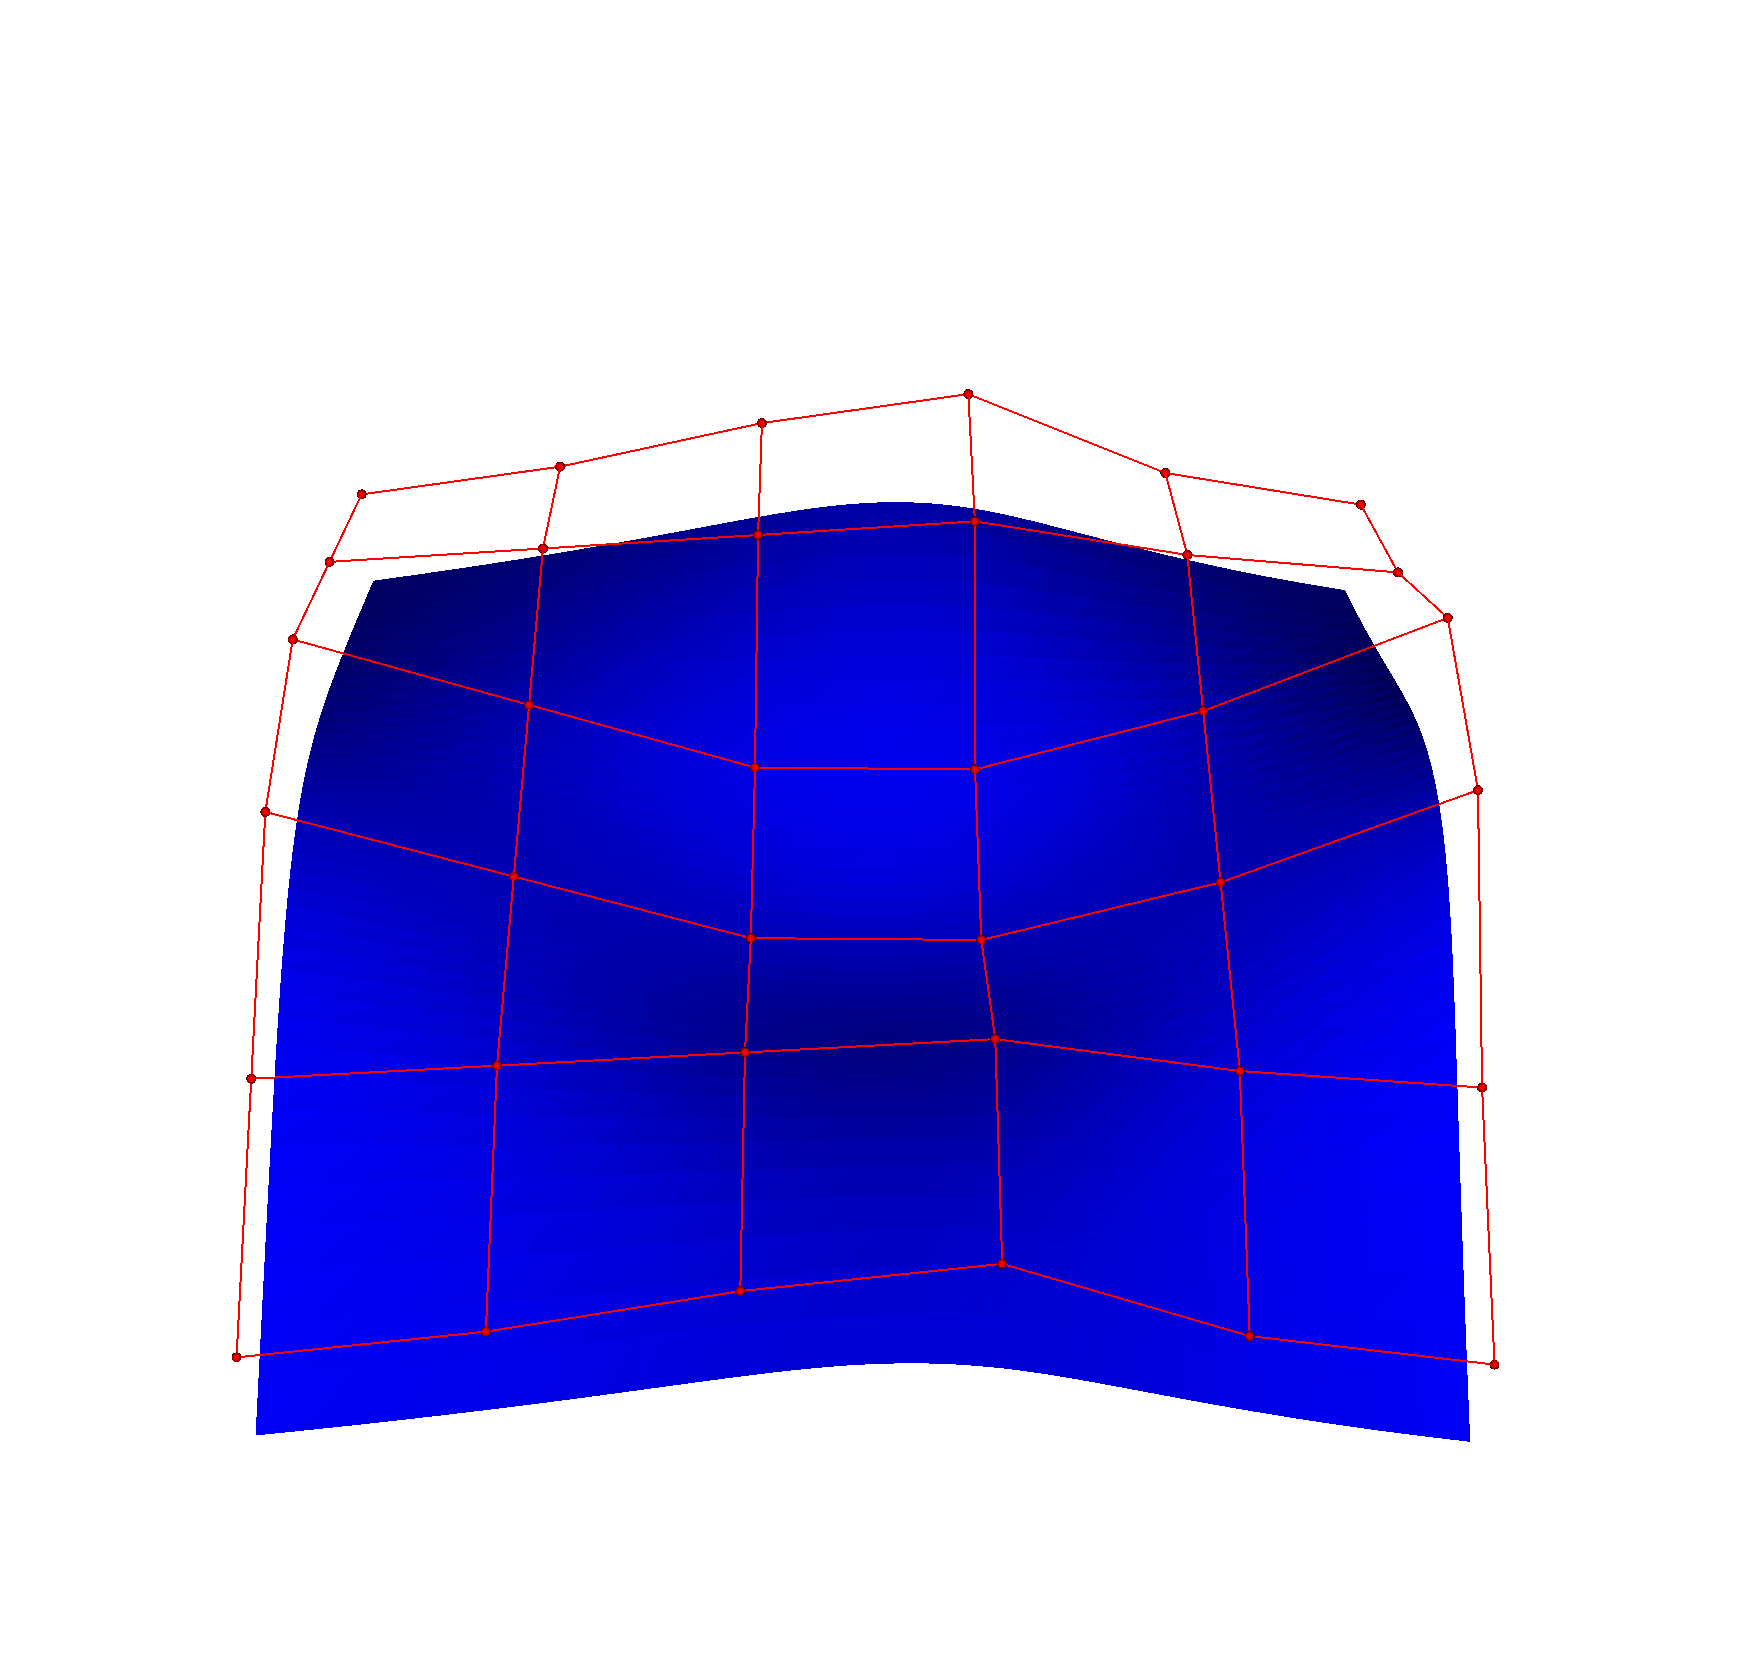
\includegraphics[height=\textwidth, trim=90 90 90 90, clip]{figures/registration/splines/spline2.png}
    % \end{subfigure}
    \begin{subfigure}[b]{0.49\textwidth}
        \centering
        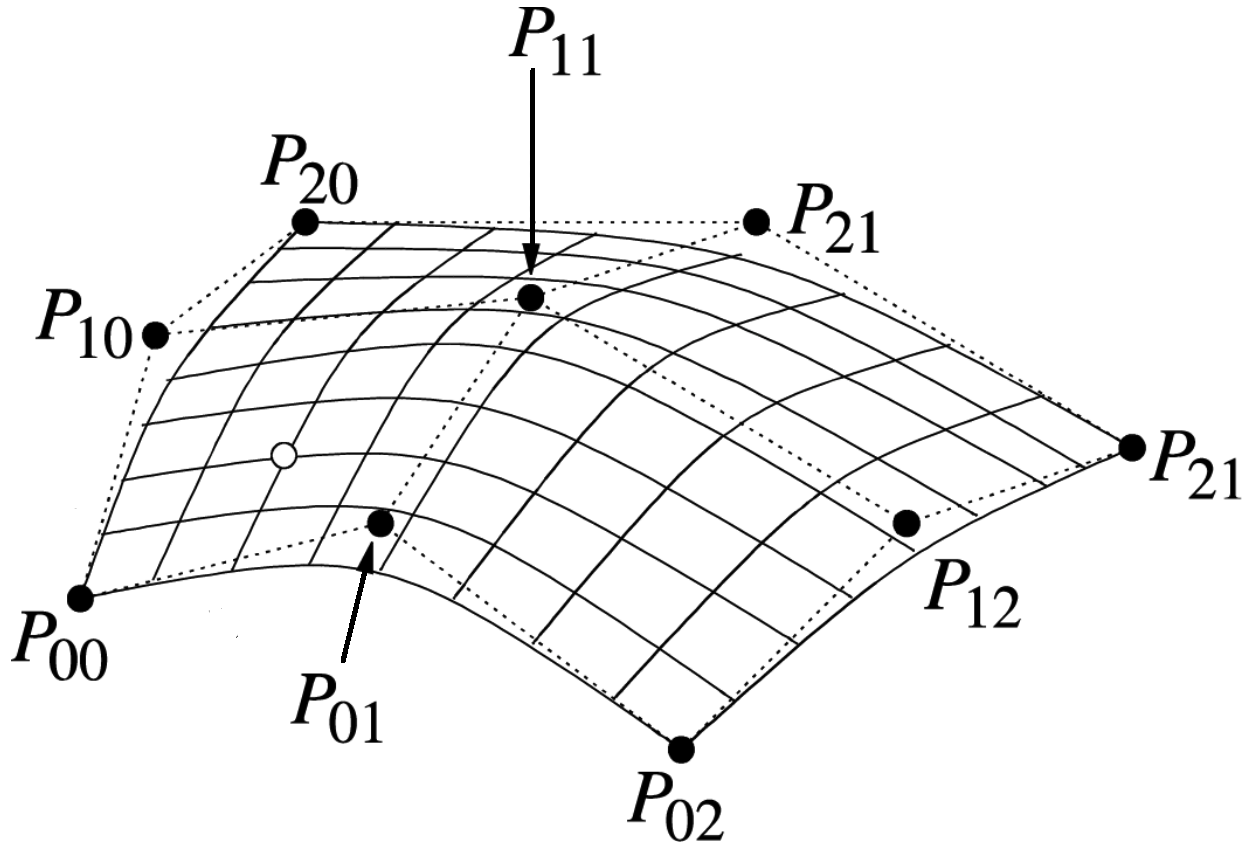
\includegraphics[height=.6\textwidth]{figures/registration/splines/spline5.png}
        \caption{Bicubic spline}
        \label{fig:bicubicspline}
    \end{subfigure}
    \vskip\baselineskip
    \begin{subfigure}[b]{0.49\textwidth}
        \centering
        \begin{adjustbox}{width=.6\textwidth}
            \begin{tikzpicture}
                \tikzset{
                    ctrlpoint/.style={%
                            draw=black,
                            fill,
                            circle,
                            inner sep=0,
                            minimum width=3pt,
                        }
                }
                \newcommand\Bezier[4]{% \bezier (lowercase 'b') was already defined elsewhere
                    \node (p1) [ctrlpoint,label=90:$P_1$] at (#1) {};
                    \node (p2) [ctrlpoint,label=90:$P_2$] at (#2) {};
                    \node (p3) [ctrlpoint,label=90:$P_3$] at (#3) {};
                    \node (p4) [ctrlpoint,label=90:$P_4$] at (#4) {};
                    \draw [black, dotted] (p1) -- (p2) -- (p3) -- (p4);
                    \draw [black] (#1) .. controls (#2) and (#3) .. (#4);
                }
                \Bezier{0,0}{1,1}{2,-1}{3,0}
            \end{tikzpicture}
        \end{adjustbox}
        \caption{Cubic spline}
        \label{fig:cubicspline}
    \end{subfigure}

    % \begin{subfigure}[b]{0.49\textwidth}
    %     \centering
    %     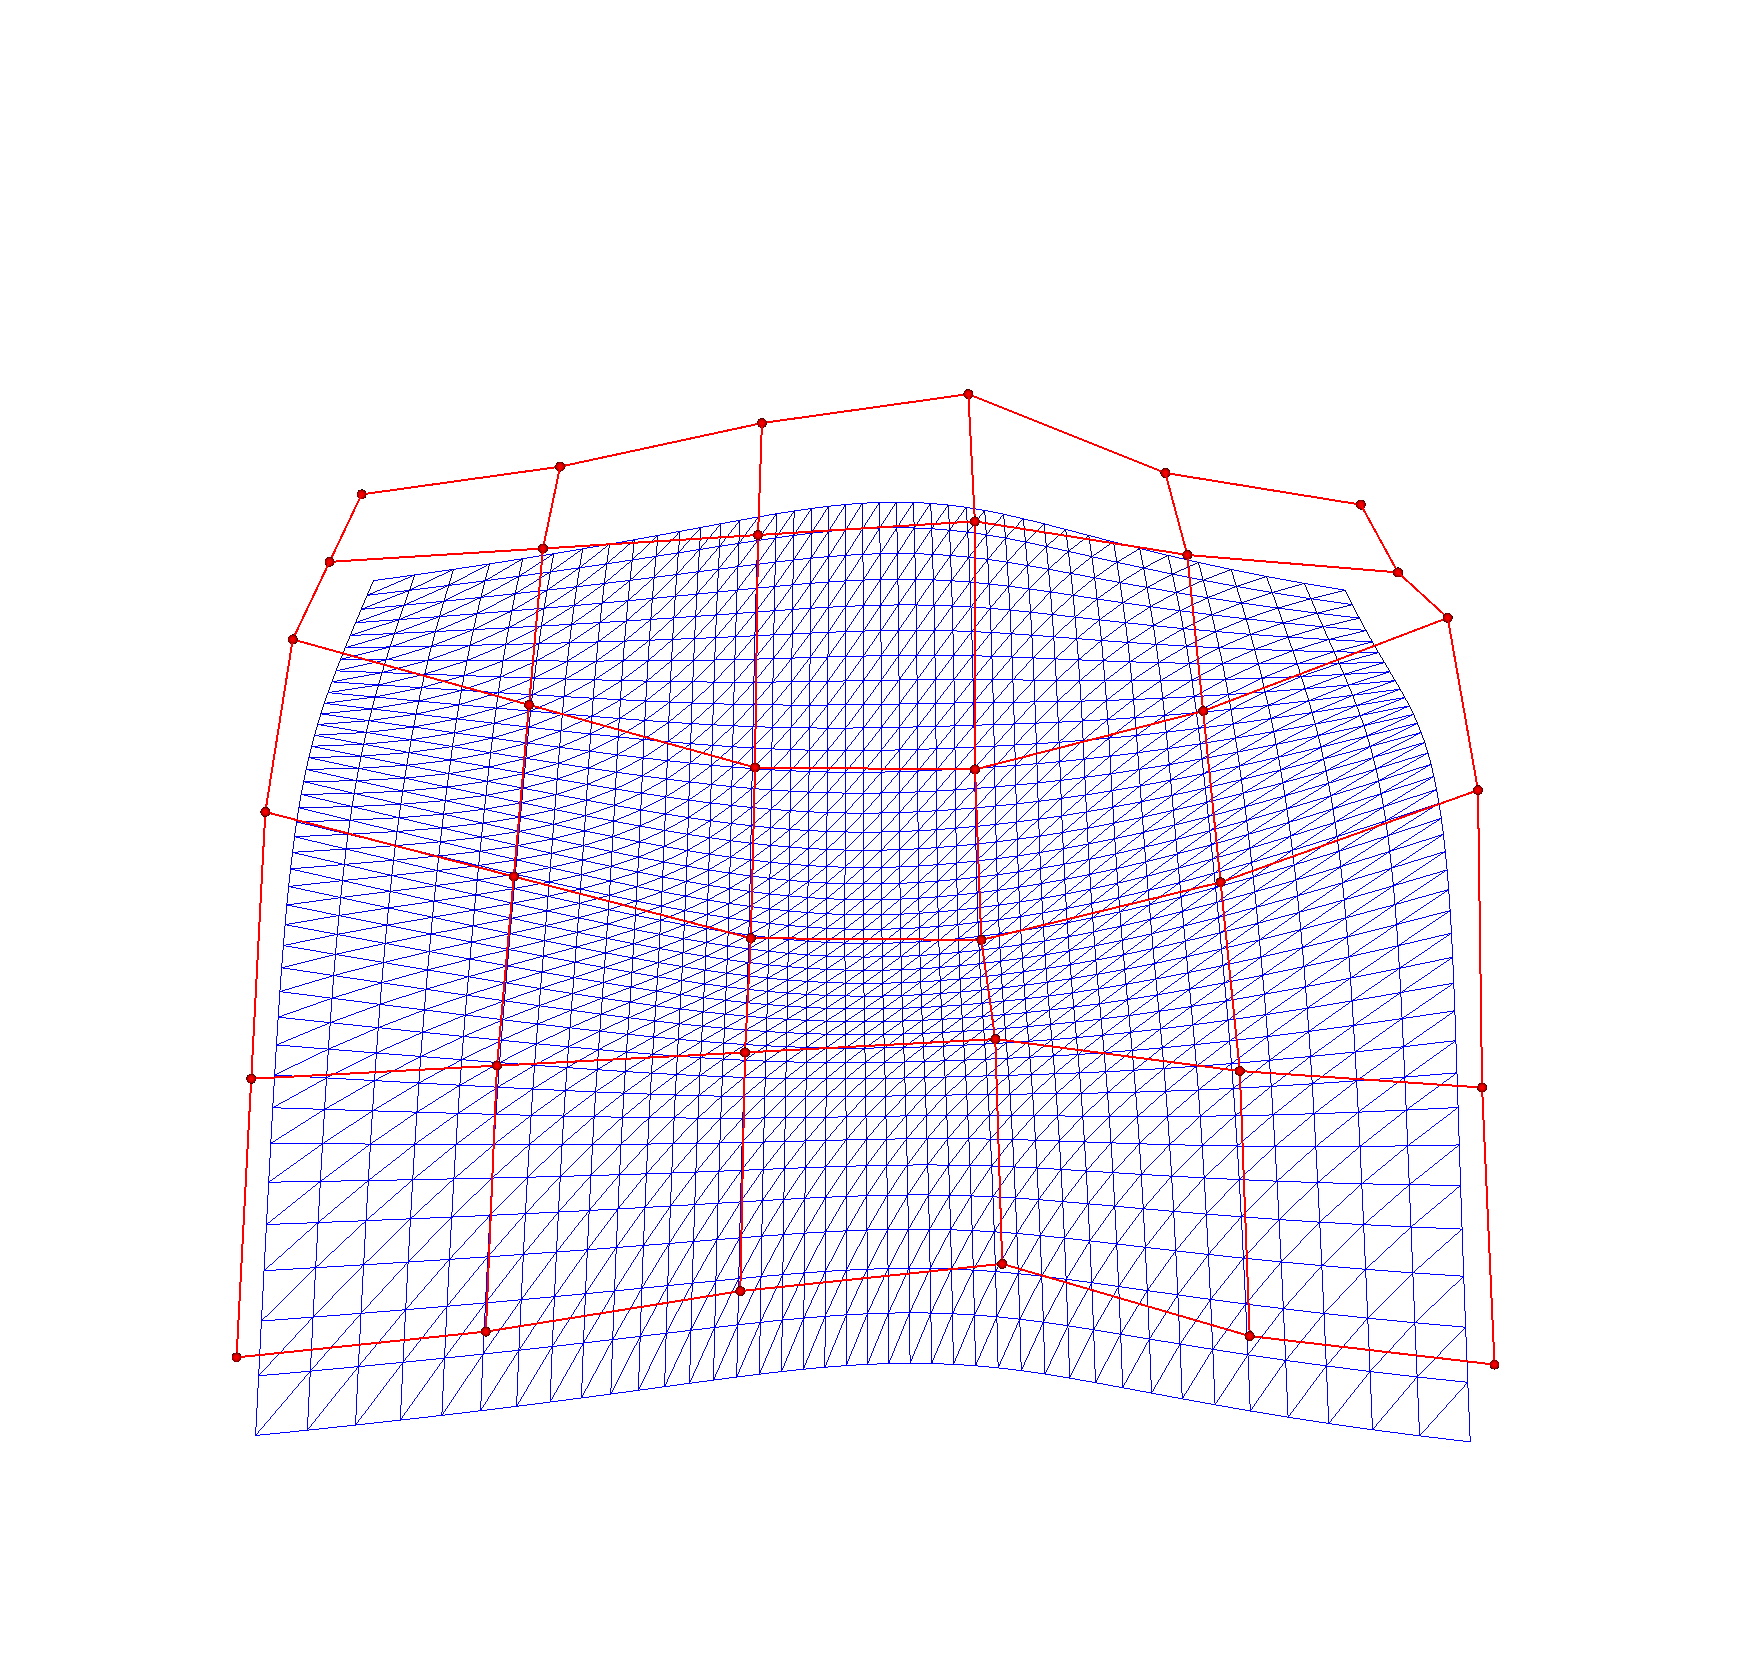
\includegraphics[height=\textwidth, trim=90 90 90 90, clip]{figures/registration/splines/spline3.png}
    % \end{subfigure}
    \caption{Splines with control points emphasized.}
    \label{fig:spline}
\end{figure}